\documentclass[11pt]{article}
\usepackage[margin=1in]{geometry}
\usepackage[scaled=0.92]{helvet}\renewcommand{\familydefault}{\sfdefault}
\usepackage[T1]{fontenc}
\usepackage{xcolor,listings,booktabs,array,enumitem,graphicx}
\usepackage[colorlinks=true,linkcolor=blue!55!black,urlcolor=blue!55!black]{hyperref}
\definecolor{ink}{HTML}{1F1F1E}\definecolor{codebg}{HTML}{F4F3EF}\definecolor{kw}{HTML}{1F5AA6}\definecolor{cm}{HTML}{6B6A64}\definecolor{st}{HTML}{1A7F5A}
\color{ink}
\lstset{language=Python, basicstyle=\ttfamily\small, keywordstyle=\color{kw}\bfseries, commentstyle=\color{cm}\itshape, stringstyle=\color{st},
  backgroundcolor=\color{codebg}, frame=none, xleftmargin=6pt, xrightmargin=6pt, aboveskip=6pt, belowskip=6pt, columns=fullflexible, keepspaces=true,
  showstringspaces=false, breaklines=true, upquote=true}
\lstdefinestyle{out}{language={}, basicstyle=\ttfamily\small\color{cm}, backgroundcolor=\color{white}, frame=leftline, rulecolor=\color{kw!40}, keywordstyle={}, stringstyle={}}
\lstdefinestyle{sh}{language=bash, keywordstyle=\color{kw}}
\newcolumntype{L}[1]{>{\raggedright\arraybackslash}p{#1}}
\setlist{itemsep=2pt,topsep=3pt}
\setlength{\parindent}{0pt}\setlength{\parskip}{5pt}
\title{\textbf{scKQE-2 tutorial}\\[3pt]\large Reproducible quantum clustering of single-cell data on the whole transcriptome}
\author{Henry Han\\ \small Data Science and AI Innovation Laboratory, Baylor University, Waco, TX 76798, USA\\ \small \texttt{hank08819@gmail.com}\\[4pt] \small scKQE-2 version 1.0.0}
\date{}
\begin{document}
\maketitle
\vspace{-12pt}

scKQE-2 clusters single-cell RNA-seq data on the whole transcriptome through a reproducible quantum encoding. In one sentence, it turns each cell into a quantum state that holds all of its genes and groups cells whose states are close. No step is trained and no step draws a random number, so the same counts give the same clusters on every run.

This tutorial goes from a count matrix to clusters, markers and a reproducibility check. The complete script is \texttt{examples/tutorial.py}. The outputs shown in gray come from running it on a public atlas of 100,000 mouse embryo cells (Theiler stages 14 to 27, 74 embryos).

\begin{figure}[h]
\centering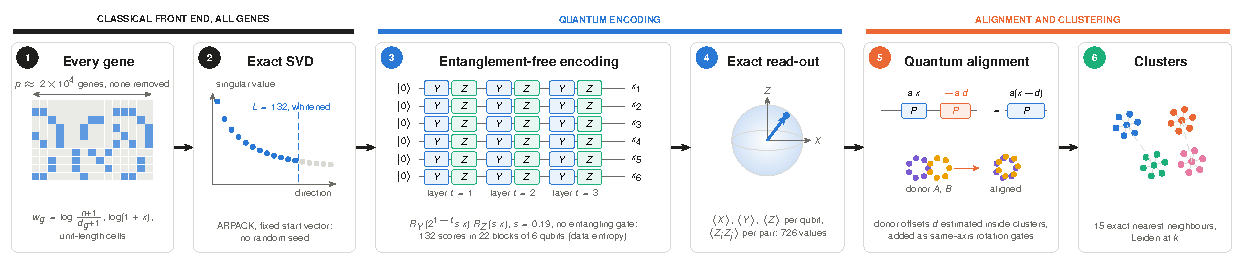
\includegraphics[width=\textwidth]{figs/pipeline.pdf}
\caption{\textbf{The six steps of scKQE-2.} The whole transcriptome enters an exact decomposition with no random seed; each of the 132 scores is encoded on its own qubit, in blocks of 6 qubits with no entangling gate; the exact read-out of every qubit forms the features; donor correction (step 5) is optional; a nearest-neighbor graph is partitioned by Leiden.}
\end{figure}

\section{Install}
\begin{lstlisting}[style=sh]
pip install scKQE2              # CPU
pip install "scKQE2[gpu]"       # with PyTorch for the GPU backend
\end{lstlisting}
scKQE-2 needs Python 3.9 or later, \texttt{scanpy}, \texttt{anndata}, \texttt{umap-learn}, \texttt{igraph} and \texttt{leidenalg}. A CUDA GPU with PyTorch speeds up the encoding and the nearest-neighbor search; without one, both run on the CPU and give the same clusters.

\section{Prepare the data}
scKQE-2 reads \textbf{raw counts} (integers), not normalized values. It takes them from \texttt{adata.raw.X} when it exists, otherwise from \texttt{adata.X}, or from a layer named with \texttt{layer=}. You also need the number of clusters $k$. With an annotation, use the number of annotated types; the labels are used for nothing else.
\begin{lstlisting}
import anndata as ad
import sckqe2

adata = ad.read_h5ad("atlas.h5ad")
y = adata.obs["cell_type"].astype(str)
keep = ~y.isin(["unknown", "nan"])              # drop unannotated cells
counts = y[keep].value_counts()
keep &= y.isin(counts.index[counts >= 10])     # drop types with fewer than 10 cells
adata = adata[keep.values].copy()
k = adata.obs["cell_type"].nunique()
\end{lstlisting}
\begin{lstlisting}[style=out]
100000 cells, 45525 genes, 31 annotated types
\end{lstlisting}

\section{Choose the gene set}
scKQE-2 uses the whole transcriptome by default. On atlases whose signal is concentrated in few directions compared with the number of clusters, 5,000 highly variable genes work better. A label-free rule decides: it measures the data entropy $h_{\mathrm{PA}}$ of the signal directions on 10,000 cells and computes $\Delta = h_{\mathrm{PA}} - \log_2 k$. If $\Delta > 1.15$ the rule chooses 5,000 HVGs, otherwise the whole transcriptome.
\begin{lstlisting}
X = adata.raw.X if adata.raw is not None else adata.X
gene_set, delta, h_pa, n_signal = sckqe2.choose_gene_set(X, k)
\end{lstlisting}
\begin{lstlisting}[style=out]
Delta = 1.69 (h_PA = 6.64, 111 signal directions) -> gene set: hvg5000
\end{lstlisting}

\section{Cluster}
\begin{lstlisting}
model = sckqe2.kqe2(adata, n_clusters=k, gene_set=gene_set)
\end{lstlisting}
\begin{lstlisting}[style=out]
31 clusters in 65 s; features (100000, 726)
\end{lstlisting}
The call writes three outputs into \texttt{adata}:

\begin{tabular}{@{}L{4.2cm}L{11cm}@{}}
\toprule
Output & Content\\
\midrule
\texttt{adata.obsm["X\_kqe2"]} & quantum features of every cell (726 per cell with the default settings)\\
\texttt{adata.obs["kqe2"]} & cluster of every cell\\
\texttt{adata.uns["kqe2"]} & every parameter used, and the Leiden resolution that gave $k$ clusters\\
\bottomrule
\end{tabular}

Inside, the steps are: IDF-weighted log counts of the whole transcriptome; an exact decomposition into 132 directions (ARPACK from a fixed start vector, no random seed); a quantum encoding of each direction on its own qubit, in blocks of 6 qubits with no entangling gate; a 15-nearest-neighbor graph; and Leiden at $k$ clusters.

\paragraph{What scKQE-2 does to the counts.} It applies one fixed transformation, with nothing to choose:
\begin{enumerate}
\item $\log(1 + \mathrm{count})$ for every gene of every cell;
\item each gene is multiplied by its IDF weight, $\log\big((m+1)/(d+1)\big)$ divided by the largest such value, where $m$ is the number of cells and $d$ the number of cells that detect the gene; genes seen in few cells, as the markers of rare types are, receive more weight;
\item each cell is scaled to unit length, which reduces the effect of sequencing depth.
\end{enumerate}
In the 5,000-HVG mode, each cell is instead scaled to 10,000 counts before the logarithm, and no IDF weight is used. scKQE-2 does not scale genes, regress out covariates or correct batches; donor correction is optional (Section~\ref{sec:align}).

With an annotation you can score the clusters; the labels enter only here:
\begin{lstlisting}
from sklearn.metrics import adjusted_mutual_info_score
adjusted_mutual_info_score(adata.obs["cell_type"], adata.obs["kqe2"])
\end{lstlisting}
\begin{lstlisting}[style=out]
0.6569
\end{lstlisting}

\begin{figure}[h]
\centering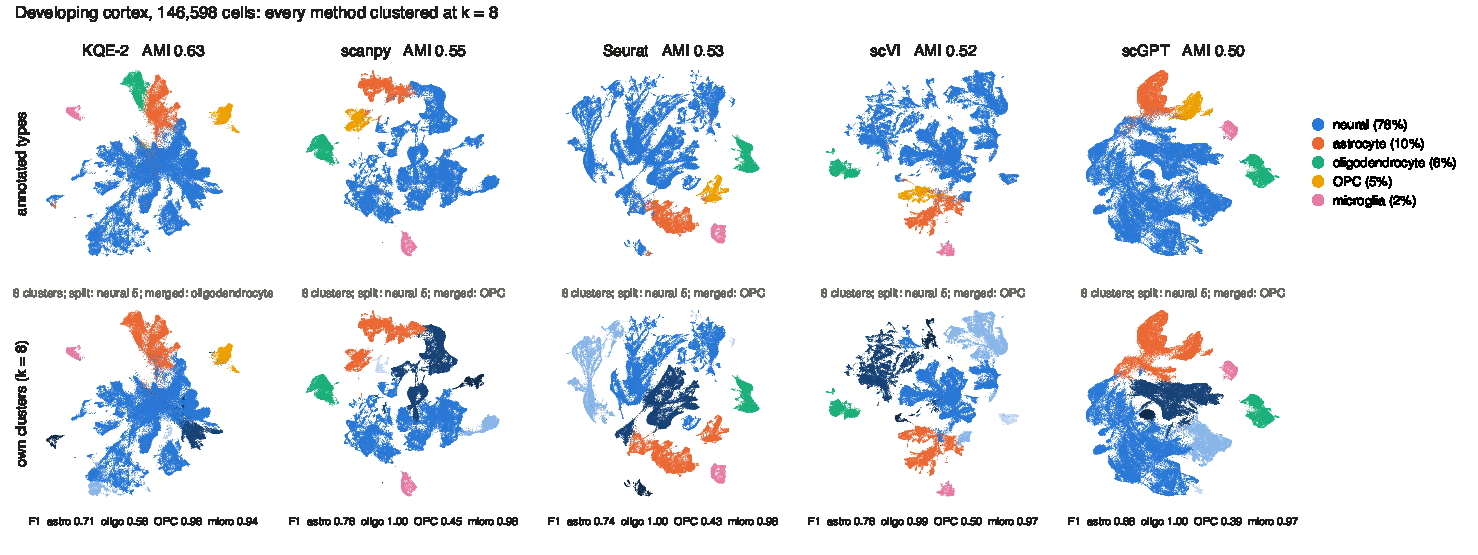
\includegraphics[width=\textwidth]{figs/devcortex_k8.pdf}
\caption{\textbf{What the clusters look like.} Developing cortex, 146,598 cells, every method clustered at eight clusters. Top: UMAP of each embedding colored by annotated type; bottom: each method's own clusters. scKQE-2 (left) is the only method that gives the oligodendrocyte precursor cells (OPC) their own cluster (F1 0.96, against 0.39 to 0.50).}
\end{figure}

\section{Check reproducibility}
\begin{lstlisting}
import numpy as np
features, clusters = adata.obsm["X_kqe2"].copy(), adata.obs["kqe2"].values.copy()
sckqe2.kqe2(adata, n_clusters=k, gene_set=gene_set)        # run again
np.array_equal(features, adata.obsm["X_kqe2"]), np.array_equal(clusters, adata.obs["kqe2"].values)
\end{lstlisting}
\begin{lstlisting}[style=out]
(True, True)
\end{lstlisting}
Both are true by construction: there is no training seed and no random sampling, and Leiden uses a fixed seed (\texttt{leiden\_seed=0}).

\section{Downstream analysis with scanpy}
The quantum features plug into any scanpy workflow, for example a UMAP and the markers of every cluster on the whole transcriptome:
\begin{lstlisting}
import scanpy as sc
sc.pp.neighbors(adata, use_rep="X_kqe2", n_neighbors=15, random_state=0)
sc.tl.umap(adata, random_state=0)
sc.pl.umap(adata, color=["kqe2", "cell_type"])

lognorm = adata.copy()
lognorm.var_names = lognorm.var["feature_name"].astype(str).values   # gene symbols
lognorm.var_names_make_unique()
lognorm.raw = None                    # rank on the symbol matrix, not on adata.raw
sc.pp.normalize_total(lognorm, target_sum=1e4); sc.pp.log1p(lognorm)
sc.tl.rank_genes_groups(lognorm, "kqe2", method="wilcoxon")
\end{lstlisting}
\begin{lstlisting}[style=out]
cluster 0 (mostly notochordal cells): Slit2, T, Cobl
cluster 1 (mostly epithelial cells): Nfia, Pcdh9, Meg3
cluster 2 (mostly keratinocytes): Efna5, Prtg, Sema3a
\end{lstlisting}

\section{Donor correction (optional)}\label{sec:align}
When donors are replicates of one condition, scKQE-2 can remove donor offsets deterministically (quantum alignment). It estimates each donor's offset inside clusters and subtracts it from the scores, which equals adding a rotation by the opposite angle to each gate.
\begin{lstlisting}
sckqe2.kqe2(adata, n_clusters=k, gene_set=gene_set,
            donor_key="donor_id", key_added="kqe2_aligned")
\end{lstlisting}
\begin{lstlisting}[style=out]
Not run on this atlas: its donors are embryos at Theiler stages 14 to 27,
so their differences are developmental biology, the case in which
alignment should not be used.
\end{lstlisting}
\textbf{Do not use it} when donors differ in biology that you want to keep, such as developmental age or disease status: their differences would be removed as if they were technical.

\section{Command line}
\begin{lstlisting}[style=sh]
sckqe2 atlas.h5ad --label cell_type --out clusters.csv          # gene set chosen by the rule
sckqe2 atlas.h5ad --k 25 --gene-set all --donor donor_id --out clusters.csv
\end{lstlisting}

\section{Parameters}
\begin{tabular}{@{}L{3.1cm}L{2.6cm}L{9.6cm}@{}}
\toprule
Parameter & Default & Meaning\\
\midrule
\texttt{n\_clusters} & required & number of clusters\\
\texttt{gene\_set} & \texttt{"all"} & \texttt{"all"} (IDF weighting) or \texttt{"hvg5000"} (5,000 HVGs, depth normalization)\\
\texttt{n\_directions} & 132 & directions of the exact decomposition\\
\texttt{qubits} & 6 & qubits per block\\
\texttt{scale} & 0.19 & rotation angle per unit score\\
\texttt{n\_neighbors} & 15 & nearest neighbors of the graph\\
\texttt{tol} & $10^{-6}$ & convergence tolerance of the decomposition\\
\texttt{backend} & \texttt{"statevector"} & \texttt{"statevector"} (the implementation of the paper, GPU when available) or \texttt{"closed\_form"} (float64 formulas)\\
\texttt{leiden\_seed} & 0 & seed of Leiden\\
\texttt{donor\_key} & None & obs column with donors; enables quantum alignment\\
\bottomrule
\end{tabular}

The defaults are the settings of the paper, and we recommend keeping them.

\section{Scale and resources}
The decomposition is the longest step. On a 1,120,336-cell atlas with 32,031 genes, the embedding took 973 s on one NVIDIA RTX A6000 GPU with a peak memory of 13.2 GB; the decomposition took 949 s of this time and the quantum encoding 18 s. Atlases of up to 2.1 million cells have been clustered on one GPU.

\section{Frequently asked questions}
\textbf{Why does it need the number of clusters?}\\*
Leiden is run at the resolution that gives exactly $k$ clusters, the protocol under which methods are compared fairly. Without an annotation, choose $k$ from biology or try several values; the result for each $k$ is reproducible.

\textbf{Without entanglement, is scKQE-2 still quantum?}\\*
Yes. Every cell is encoded as a quantum state, its features are expectations of quantum observables, the cells are clustered in quantum-state space, and the same circuit runs on quantum hardware, where every measured feature can be checked against its exact value. Entangling gates would enlarge the space of representations, but they spread noise between qubits and make exact evaluation infeasible, so features would be estimated from a finite number of measurements and change from run to run. For single-cell atlases, whose clusters decide the markers, pathways and drug targets, that price is unaffordable: scKQE-2 keeps the quantum representation and leaves out the noise.

\textbf{Why not use entangling gates?}\\*
Because removing them is what makes the results exact and reproducible, at no cost in accuracy. Without entangling gates every feature is an exact formula of one score, computed in time linear in the number of qubits, and the fidelity of two cells becomes a product over qubits, which makes clustering a million cells possible. A perturbation of one score, or a hardware error on one qubit, then moves only that qubit's features; the paper proves that removing entanglement is necessary and sufficient for this locality. With entangling gates, exact evaluation is \#P-hard in general and errors spread across qubits. In 42 comparisons on our atlases, the circuit with entangling gates was within 0.01 AMI of the circuit without them in 31 and ahead in 6 of the rest: entanglement bought no accuracy.

\textbf{Why is this quantum clustering reproducible, unlike traditional quantum models?}\\*
Traditional quantum models lose reproducibility at three points, and scKQE-2 removes each of them. First, they train their circuits from random initial parameters, and the trained circuit differs from run to run; scKQE-2 uses a fixed circuit and trains nothing. Second, they estimate every feature from a finite number of measurements, so each estimate carries shot noise, and the result depends on the calibration of the device on that day; scKQE-2 evaluates every feature exactly. Third, their entangling gates make exact evaluation infeasible, so a result cannot be recomputed and checked; scKQE-2 has no entangling gate, so every feature has a closed form. The steps around the circuit are deterministic as well: the decomposition starts from a fixed vector and Leiden uses a fixed seed. The same counts therefore give bit-identical features and the same clusters on every run.

\textbf{Why are the results identical across runs while scVI or scGPT change?}\\*
scKQE-2 has no training and no random gene sampling, and its decomposition starts from a fixed vector and converges to the same answer. Models that are trained or that sample genes at random give different clusters with every seed.

\textbf{Do the two backends give the same features?}\\*
They agree within $2 \times 10^{-5}$ on real data; \texttt{"statevector"} reproduces the published results bit for bit.

\textbf{Does it need a GPU?}\\*
No. Without a CUDA GPU the encoding and the nearest-neighbor search run on the CPU and give the same clusters. A GPU shortens these two steps; the exact decomposition runs on the CPU in both cases.

\textbf{Can I give it normalized or log-transformed data?}\\*
No. scKQE-2 expects raw counts, because it applies its own weighting and log transform to every gene. If \texttt{adata.X} holds normalized values, pass the counts with \texttt{layer="counts"} or keep them in \texttt{adata.raw}.

\textbf{Why 6 qubits and 132 directions?}\\*
The number of qubits per block follows from the data entropy of the signal directions, which ranges from 5 to 7 bits on the atlases studied; 6 is used everywhere. The 132 directions exceed the number of signal directions found by parallel analysis on every atlas tested, so no signal is cut. Both defaults are the settings of the paper.

\textbf{When should I use quantum alignment rather than Harmony?}\\*
Use quantum alignment when you need a donor correction that gives the same result on every run: it draws no random number, whereas Harmony's soft clustering depends on its seed. Use either only when donors are replicates of one condition.

\textbf{Can I run the circuit on a quantum computer?}\\*
Yes. Without entangling gates the circuit needs only single-qubit rotations, and every measured feature can be compared with its exact value. A quantum processor is much slower than the exact evaluation (seconds per cell against microseconds), so atlas-scale analyses use the exact evaluation.

\textbf{Which data does it support?}\\*
Single-cell and single-nucleus RNA-seq count matrices from droplet-based and combinatorial-indexing protocols, from human, mouse and zebrafish, as long as raw counts are available. It has been run on atlases from tens of thousands to 2.1 million cells.

\end{document}
